\section{Ejercicio 2: Construyendo Reportes en Power BI - Tarea 1: Crear un Grafico} 

1. En Power BI Desktop, en la barra derecha de navegación, hacer click en Reporte (Report).\\
2. En el panel de Visualizaciones (Visualizations), hacer click en Gauge.\\
3. Arrastar el campo (LineTotal) de la table (Sales) a la propiedad Valor (Value) del objeto gauge.\\
4. Arrastrar la medida Drag the TargetSales measure from the Sales table to the Target value property of the
gauge.\\
5. Click Format, expand Gauge axis, and then in the Max box, type 146000.\\
6. Expand Title, in the Title Text box, type Target Sales, and then click Center.\\

	\begin{center}
	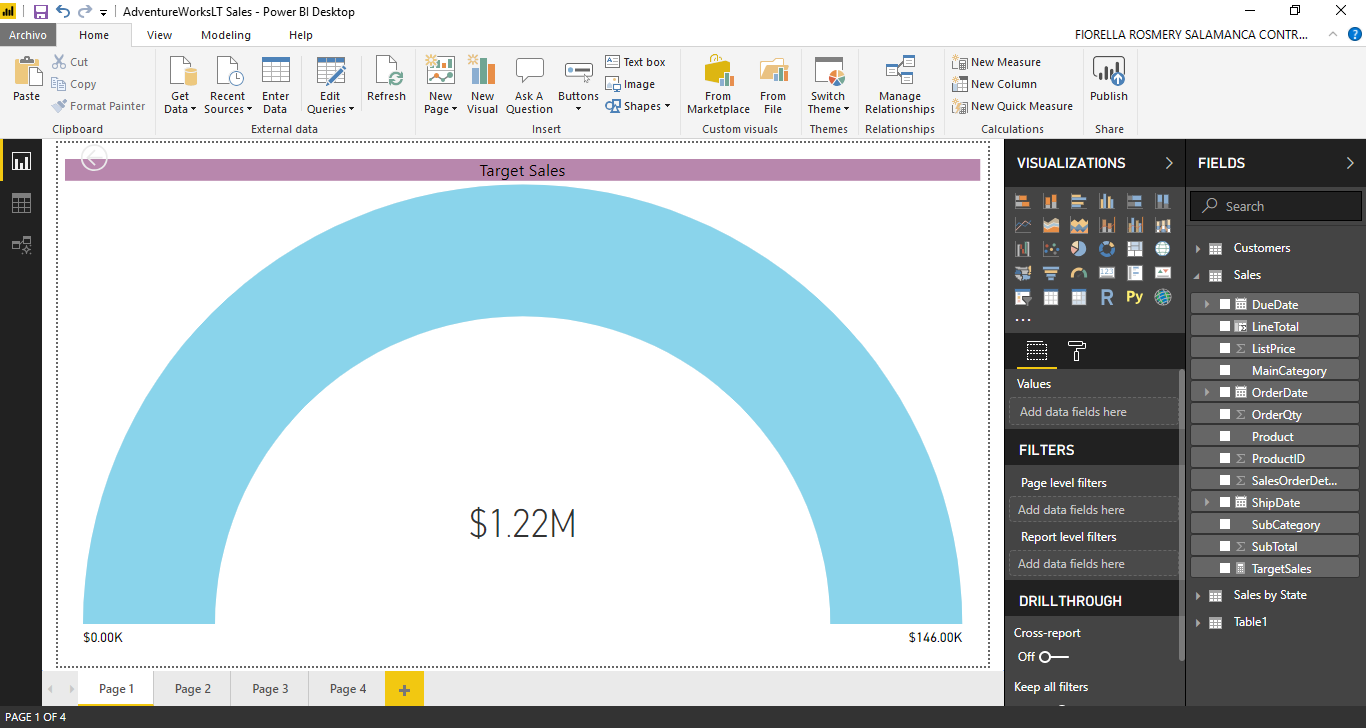
\includegraphics[width=17cm]{./Imagenes/Ejercicio2/Tarea1/1}
	\end{center}	

7. Click the report canvas, and then drag the CompanyName field from the Customers table onto the
report. Power BI automatically creates a table.\\
8. Drag the LineTotal field from the Sales table onto the report.\\
9. Make sure that the table has focus, and then in the Visualizations pane, click Pie chart.\\
10. Expand the chart to make all of the company names visible by using the resizer handles on the edge
of the chart.\\
11. With the focus still on the pie chart, click Format, and then expand Title.\\
12. In the Title Text box, type Top Selling Customers, and then click Center.\\

	\begin{center}
	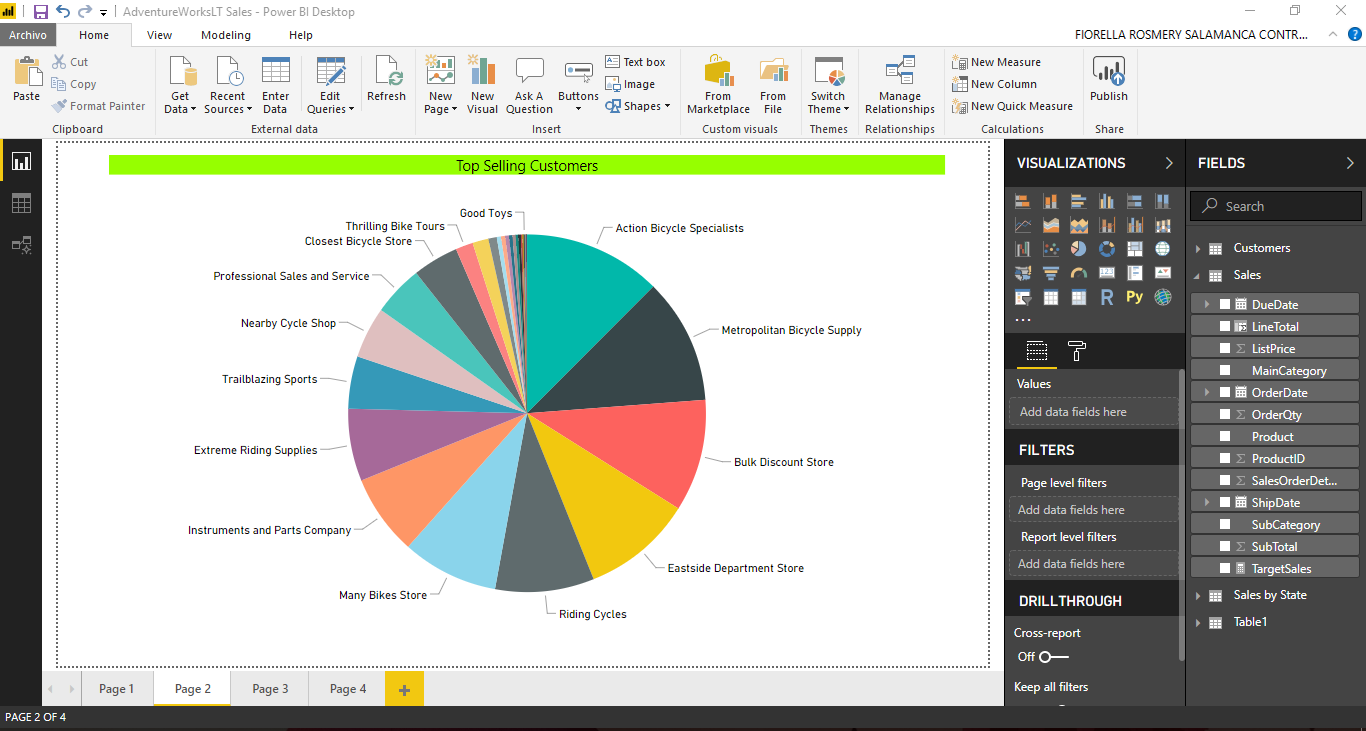
\includegraphics[width=17cm]{./Imagenes/Ejercicio2/Tarea1/2}
	\end{center}	

13. Drag the MainCategory field from the Sales table onto the report canvas. Power BI creates a table.\\
14. Drag the OrderQty field onto the table.\\
15. In the Visualizations pane, click Stacked bar chart.\\
16. In the Visualizations pane, click Fields.\\
17. Drag the OrderQty field onto the Color saturation property. Notice that the colors change.\\
18. In the Visualizations pane, click Analytics, expand Constant Line, and then click Add.\\
19. In the Value box, type 500.\\
20. Change Color to red, toggle Data label to On, and then change the color to red.\\
21. In the Visualizations pane, click Format, and expand Title.\\
22. In the Title Text box, type Orders by Main Category, and then click Center.\\

	\begin{center}
	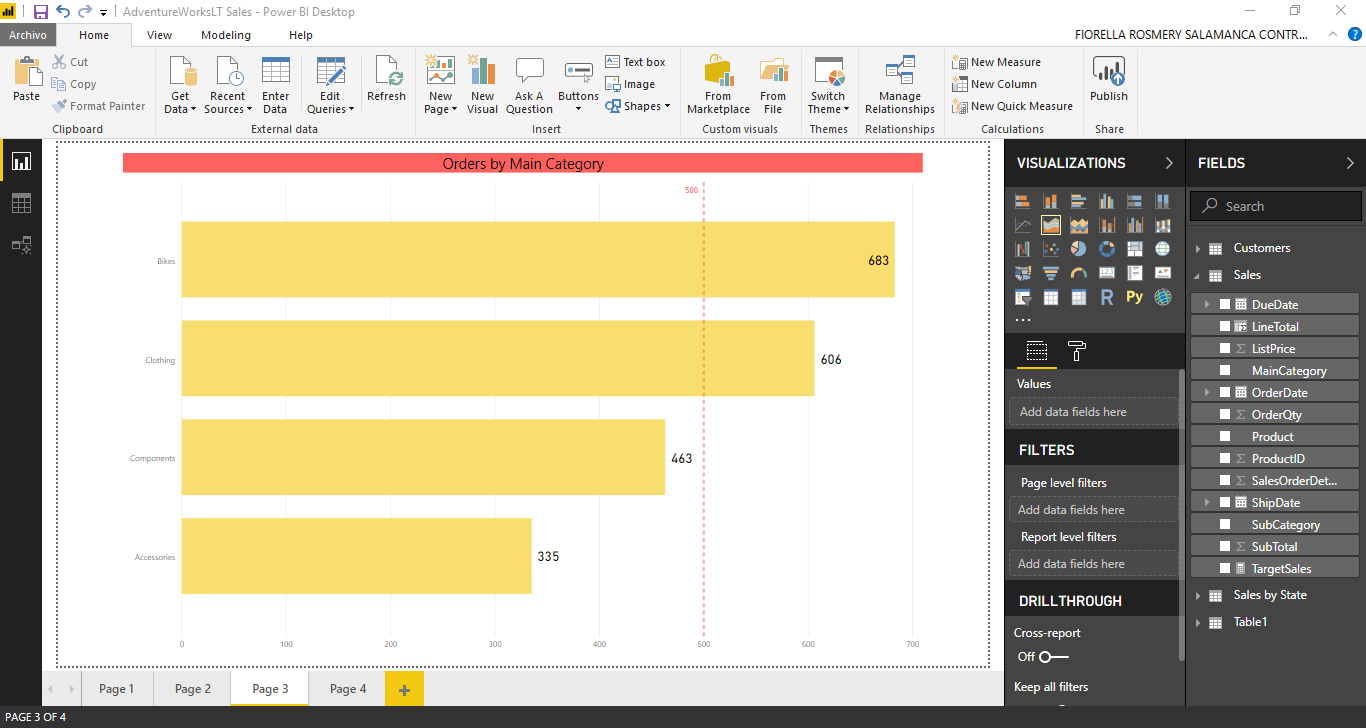
\includegraphics[width=17cm]{./Imagenes/Ejercicio2/Tarea1/3}
	\end{center}	

23. Click the report canvas to give it focus, and then in the Visualizations pane, click Donut chart.\\
24. In the Sales table, select MainCategory and LineTotal.\\
25. In the Visualizations pane, click Format, and then expand Title.\\
26. In the Title Text box, type Sales by Main Category, and then click Center.\\

	\begin{center}
	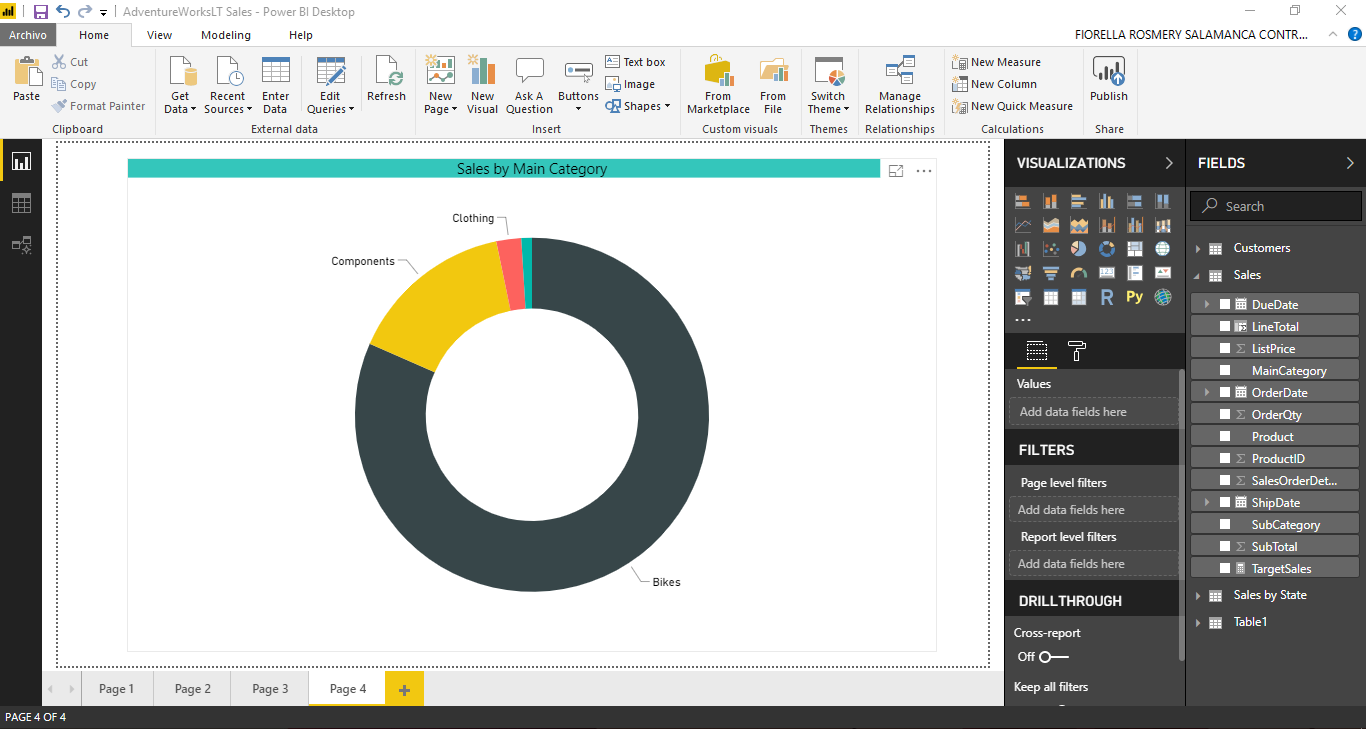
\includegraphics[width=17cm]{./Imagenes/Ejercicio2/Tarea1/4}
	\end{center}	

27. Drag the Product field from the Sales table onto the report canvas. Power BI creates a table.\\
28. Drag the LineTotal field from the Sales table onto the products table chart.\\
29. In the Sales table, select the MainCategory field.\\
30. In the Visualizations pane, click Fields.\\
31. In the Filters pane, expand LineTotal(All).\\
32. In the Show items when the value list, select is greater than, and then in the box below, type
32000.\\
33. Click Apply filter.\\
34. Expand MainCategory(All), and then select Bikes.\\
35. In the Visualizations pane, click Stacked column chart.\\
36. In the Visualizations pane, click Format, and then expand Title.\\
37. In the Title Text box, type Top 10 Selling Bikes, and then click Center.\\

	\begin{center}
	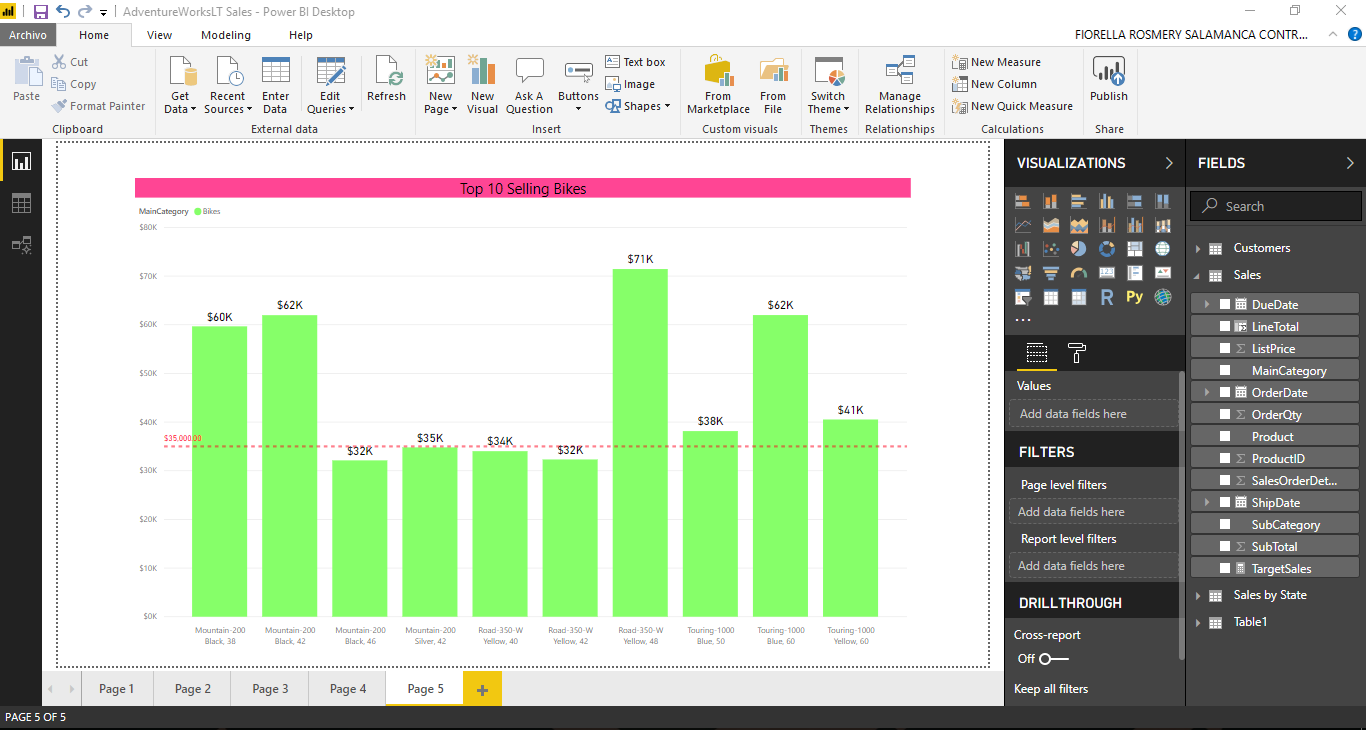
\includegraphics[width=17cm]{./Imagenes/Ejercicio2/Tarea1/5}
	\end{center}	

38. In the Visualizations pane, click Analytics, expand Constant Line, and then click Add.\\
39. In the Value box, type 35000, and then set Color to red.\\
40. Toggle Data label to On, and then set Color to red.\\
41. Expand the chart to fill the remaining space on the report canvas. If necessary, move your visuals
around to make them fit.\\
42. Click Save.\\